% !TEX root = ../main.tex
%
\chapter{Results}
\label{sec:result}

This section presents the findings of the user study conducted to assess the usability of the application.
First, the results of the quantitative user experience questionnaire are presented, which allows for an evaluation of the user experience as a whole.
Subsequently, the results of the qualitative user testing are analysed in order to provide more detailed insights into the usability of the application.
Finally, the results are integrated and discussed in detail.

\section{User Experience Questionnaire}
\label{sec:result:ux}

Despite the relatively small sample size of 10 participants, the results of the User Experience Questionnaire (UEQ) provide a good overview of the overall user experience.
The scores for the different scales of the UEQ are presented in Figure~\ref{fig:ueq-1}. 

\begin{figure}[htb]
  \centering
	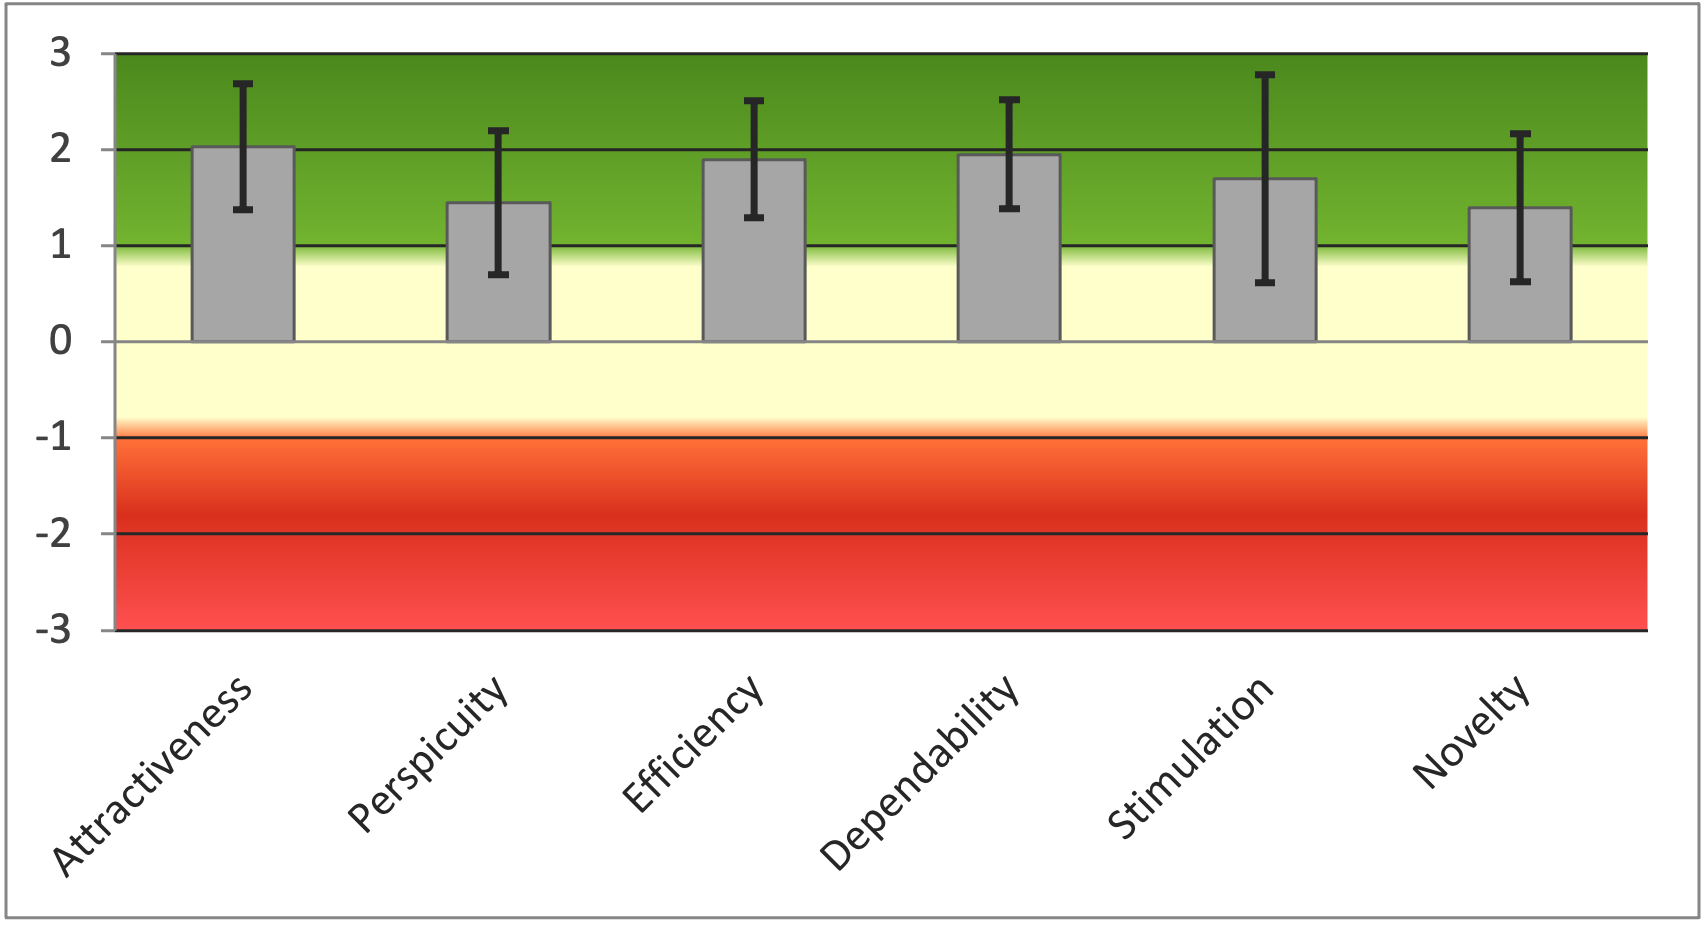
\includegraphics[width=.7\textwidth]{figures/ueq-1.png}
	\caption{Results of the User Experience Questionnaire, showing the average scores for each scale and their 95 \% confidence interval.}
  \label{fig:ueq-1}
\end{figure}

The \emph{Novelty} scale scores the lowest with a value just below 1, while the \emph{Attractiveness} scale has the highest score with 1.98.
The other scales score between 1.5 and 1.8, indicating a generally positive user experience.

The UEQ scores can be benchmarked against the results of 452 other studies provided by the UEQ benchmark.
The benchmarking results are shown in Figure~\ref{fig:ueq-2}, where \emph{Attractiveness} and \emph{Dependability} classify as \emph{Excellent}, placing them in the top 10\% of all studies.
\emph{Stimulation} and \emph{Efficiency} are classified as \emph{Good}, while \emph{Novelty} and \emph{Perspicuity} only classify as \emph{Above Average}.

\begin{figure}[htb]
	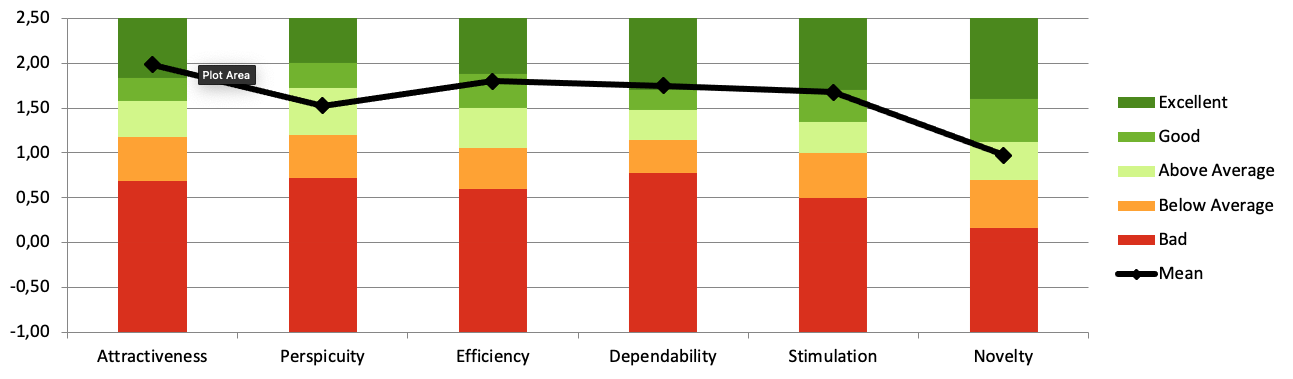
\includegraphics[width=\textwidth]{figures/ueq-2.png}
  \caption{Benchmarking results of the User Experience Questionnaire, comparing the results of the study to a benchmark of 452 other studies.}
  \label{fig:ueq-2}
\end{figure}

The variance of the scores is relatively high, which may be attributed to the limited sample size.
The variance across the first five scales ranges from 0.49 to 0.92, only exceeding 1 for the \emph{Novelty} scale with a value of 1.31.

Table \ref{tab:ueq-summary} provides a summary of the UEQ results, including mean values, confidence intervals, and standard deviation.
The standard deviation is a measure of the degree of agreement among participants, with lower values indicating higher level of agreement.
Any value below 0.83 is considered to indicate \emph{high agreement}, while values between 0.83 and 1.01 are considered \emph{medium agreement} and values above 1.01 are considered \emph{low agreement}.
Of the six scales, three exhibit high agreement, two have a medium agreement and one has a low agreement.

\begin{table}[htb]
  \centering
  \begin{tabularx}{\textwidth}{|X|l|l|l|l|l|}
  \hline
      \textbf{Scale} &  \textbf{Mean}  &  \textbf{Conf.} &  \textbf{Conf. Int.} &  \textbf{Std. Dev.} & \textbf{Agreement}\\ \hline
      \textbf{Attractiveness} & 1.983  & 0.445 & 1.538 - 2.428 & 0.718 & high \\ \hline
      \textbf{Perspicuity} & 1.525 & 0.573 & 0.952 - 2.098 & 0.924 & medium\\ \hline
      \textbf{Efficiency} & 1.800 & 0.500 & 1.300 - 2.300 & 0.806 & high \\ \hline
      \textbf{Dependability} & 1.750 & 0.432 & 1.318 - 2.182 & 0.691 & high \\ \hline
      \textbf{Stimulation} & 1.675 & 0.594 & 1.081 - 2.269 & 0.958 & medium \\ \hline
      \textbf{Novelty} & 0.975 & 0.710 & 0.265 - 1.685 & 1.145 & low \\ \hline
  \end{tabularx}
  \vspace{6pt}
  \caption{Summary of the User Experience Questionnaire results}
  \label{tab:ueq-summary}
\end{table}

\subsection*{Summary}

The analysis of the UEQ results provides insights into the application's user experience.
High scores in \emph{Attractiveness} and \emph{Efficiency} scales, accompanied by high agreement among participants, suggest that these aspects of the application are both effective and appealing.
The consistency of these scores suggests that such attributes can be rapidly gauged by users, even within the limited timeframe of the user study, leading to a uniformly positive perception.

The lower score and agreement on the \emph{Novelty} scale indicate that the perceptions of the application's innovativeness are varied.
This could be interpreted to suggest that while the application may not introduce new features or functionalities, it effectively repackages existing ones within an intuitive user interface.
The moderate novelty score may be indicative of the application's use of familiar concepts and interactions, which could reduce the learning curve by leveraging well-understood mechanisms.

However, it is important to note that these findings are based on a relatively small sample size of 10 participants.
While the results provide valuable insights, they should not be overvalued or considered definitive.
It is advisable to exercise caution in generalizing these findings without further validation from a larger, more diverse sample.

\section{Findings from Qualitative User Testing}
\label{sec:result:qualitative}

This section presents the findings from the user study conducted to evaluate the user interface of the application.
The results are organized into categories reflecting overall impressions, the learning curve and accessibility, identified issues, and recommendations for improvement, which now include feature requests.

\subsection*{Overall Impressions}
\label{sec:results:overall_impressions}

Users generally find the interface user-friendly, effective, and aesthetically pleasing, enhancing the user experience across various functionalities. 

\paragraph{User-Friendly} 
Participants highlighted the intuitive layout and ease of navigation within the interface, appreciating how straightforward it was to perform tasks without prior training or extensive help. 
\cite{P1, P2, P4, P5, P7, P8, P10}

\cleanchapterquote{So it's definitely a very nice tool, so it's pleasant to use.\footnotemark}{Participant 2}{}
\footnotetext{Also es ist auf jeden Fall sehr schönes Tool, also angenehm zum Nutzen.}
 
\paragraph{Effective} 
The effectiveness of the interface was noted in terms of its responsiveness and reliability. 
Users were satisfied with the speed at which the interface responded to commands and the consistency of its performance during tasks, which helped in building trust and reducing frustration during interactions.
\cite{P2, P4, P7, P8, P10}


\cleanchapterquote{Otherwise I thought it was super precise. I had the feeling that there wasn't much room for error.\footnotemark}{Participant 4}{}
\footnotetext{Sonst fand ich super präzise. Also ich hatte das Gefühl, da war nicht so super viel Raum für Fehler.}

\paragraph{Aesthetically Pleasing} 
Many users commented on the visual appeal of the interface, mentioning the modern and clean aesthetic that made the experience more engaging. 
\cite{P7, P8, P10}

\cleanchapterquote{In terms of design, I thought it was really cool, the way the colors are designed, even the animated background, I'm personally in favor of something like that.\footnotemark}{Participant 10}{} 
\footnotetext{Designtechnisch fand ich es echt cool, also wie die Farben gestaltet sind, auch das mit dem animierten Hintergrund, bin ich persönlich auch für sowas.}

These aspects collectively contribute to a positive user experience, making the application not only a tool that meets functional needs but also a pleasure to use, thereby encouraging repeated and prolonged engagement.

\subsection*{Learning Curve and Accessibility}
\label{sec:results:learning_curve_accessibility}

Accessibility and ease of use are the main concerns of the application, driven to reduce the technical knowledge required to enable a broader user base.
This section elaborates on the specific feedback received regarding the short comings and successes of the application in this regard.

\paragraph{Ease of Use}
As mentioned above, the overall user-friendliness was well received by participants across the board.
Feedback from users indicates that the layout and workflow of the application facilitate quick learning and ease of use.
\cite{P4, P5, P7, P8, P10}
The progress indicator, as shown in Figure~\ref{fig:design:training-section}, was particularly appreciated, as it helped users understand the current state of the application and what steps were required to complete a task.
\cite{P5, P7, P8, P9}

\cleanchapterquote{I thought it was nice that it was split into three parts, so to speak, that this overview at the top said, okay, you're currently at Step 1 and then you know, okay, there are two more to go, so you can categorize it a bit.\footnotemark}{Participant 8}{}
\footnotetext{Ich fand es schön, dass es quasi dreigeteilt war, dass diese Übersicht oben, dass da stand, okay, du befindest dich gerade bei Step 1 und dann wei{\ss}t du, okay, es folgen noch zwei weitere, dann kann man es ein bisschen einordnen.}

\paragraph{Overwhelming Aspects}
Despite the general ease of use, some users expressed concerns about overwhelming aspects of the interface.
The parameter settings often require a deep understanding of NeRF technology to understand their effects, but this did not hinder the overall usability of the application.
\cite{P5, P7}
The viewer component, while powerful, presents a steep learning curve due to its complexity and the dense presentation of information and controls. 
New users, unfamiliar with NeRF and, in particular, Nerfstudio, might find this part of the application challenging to navigate initially.
\cite{P2}

\cleanchapterquote{But the [Nerfstudio Viewer] is quite complicated in itself, I think. It would be good to have some kind of explanation next to it about what you have to do or what you can do.\footnotemark}{Participant 2}{}
\footnotetext{Der [Nerfstudio Viewer] ist aber an sich recht kompliziert, finde ich. [Es wäre gut] daneben irgendwie eine Erklärung [zu haben], was man machen muss oder was man da machen kann.}

\paragraph{Technical Complexity}
Reducing the technical complexity inherent in NeRF applications is crucial for making the application more accessible to a broader audience.
Based on the feedback received from users, who were previously unfamiliar with NeRF, the application requires users to have some level of prior knowledge.
The guided experience and the reduced number of options to configure were appreciated by certain participants.
It enabled them to quickly get started with the application without feeling overwhelmed.
Most users felt confident that after a short learning phase, they would be able to use the application effectively.
\cite{P2, P3, P4, P5, P6, P7, P8}
However, the feedback indicates a need for an onboarding process or tutorials to help new users overcome initial hurdles and gain confidence in using advanced features.
In contrast, advanced users appreciated the depth of control and customization available.
\cite{P9, P10}

\cleanchapterquote{I think I'll need a bit more time to get used to it, but I think that will happen quite quickly.\footnotemark}{Participant 2}{}  
\footnotetext{Ich glaube, ich bräuchte schon noch ein bisschen um mich rein zu arbeiten, aber ich glaube, dass das recht schnell gehen wird.}

\paragraph{Project Management}
Novice users appreciated the similarities to existing project management of an already familiar tool from the film industry. 
\cite{P5}
For experienced users, the abstraction of tedious project management tasks, like file uploads and data organization, was well received.
\cite{P1}
This allowed them to focus on the core tasks of training and rendering, without getting bogged down by administrative overhead.

\cleanchapterquote{Yes, it's definitely very self-explanatory, so how to manage projects, how to create projects, and so on. I'm familiar with this from almost all software that has something to do with film, video editing and Photoshop.\footnotemark}{Participant 5}{}
\footnotetext{Ja, ist auf jeden Fall sehr selbsterklärend, wie man also das Projektmanagement, wie man Projekte anlegt usw. Das kenne ich aus ungefähr allen Softwares, die jetzt was mit Film, mit Video Editing, Photoshop zu tun haben.}

\paragraph{Technical Language}
One particularly insightful point of concern was the unfamiliar terminology used, as there exist differences between some terms in the context of NeRF and the film industry. 
\cite{P5}
This can lead to confusion and hinder the learning process, as users struggle to understand the meaning and implications of certain terms.
Adjusting the language used in the application to specifically target the intended audience can help bridge this gap and further reduce the learning curve.

\cleanchapterquote{I think sometimes it could be less technical and a bit more translator if you make it movie-specific.\footnotemark}{Participant 5}{}
\footnotetext{Ich [finde] teilweise könnte es weniger technisch und ein bisschen mehr Übersetzter sein, wenn man das filmspezifisch macht.}

In summary, the application succeeds in providing new users with access to advanced NeRF tools, while also catering to the needs of experienced users by offering advanced options for customization.

\subsection*{Identified Issues}
\label{sec:results:issues}

The following issues were identified during the user testing sessions, based on feedback from participants. 
Most of these issues became apparent while participants were performing tasks, and then were further discussed during the post-task interviews.

\paragraph{Unclear Navigation}
Users experienced confusion about navigating through tasks and understanding their progression within the application.
This was particularly evident when having to switch to a different project.
The intended way to navigate to the dashboard was to click on the logo, which was not immediately clear to all users.
Some users succeeded in finding the dashboard after some exploration, while others used browser navigation to return to the dashboard.
\cite{P1, P4, P5, P6, P8, P10}
Some participants also mentioned uncertainties about navigating between the different sections of a project.
The progress indicator can be used to navigate between the different sections, but some users took some time to discover this feature.
\cite{P9}


\cleanchapterquote{What I would also like is for the home button to be marked with a little box when I went back, so that I know how to get back to Home.\footnotemark}{Participant 4}{}
\footnotetext{Was ich noch gerne hätte, wäre, dass der Homebutton, als ich zurückgegangen bin, also mit einem kleinen Häuschen markiert ist, damit ich wei{\ss}, wie ich zurück zu Home komme.}

\paragraph{Inconsistent Wording}
\label{sec:results:issues:inconsistent_wording}
An issue that many participants stumbled upon was the inconsistent wording used specifically on the button to start the training process.
In the version of the application used during the user study, the button was labeled \emph{"Start Processing"}, which was confusing to most users.
\cite{P2, P3, P6, P7, P8}


\cleanchapterquote{Then I would have looked somewhere on the button for 'Nerf Training' and it says 'Start Processing'.\footnotemark}{Participant 8}{}
\footnotetext{[Dann] hätte ich halt irgendwo auf dem Button nach 'Nerf Training' gesucht und da steht 'Start Processing'.}

\paragraph{Project Creation}
Similar to the wording issue, the process of creating a new project was not as intuitive as intended.
Many participants encountered a small annoyance when they tried to click on the big plus icon placed in the center of the card, which was not clickable. \fref{fig:design:dashboard}
Although everyone quickly discovered the intended way to create a new project, this issue was mentioned by almost all participants.
\cite{P3, P4, P5, P6, P7, P8}

\cleanchapterquote{If [...] I have to create a new project and there is a big plus at the top and a small plus at the bottom, I would also tend to press the big plus at first.\footnotemark}{Participant 3}{}
\footnotetext{Wenn [...] ich ein Projekt neu erstell[en] soll und oben ist ein gro{\ss}es Plus und unten ist ein kleines Plus, würde jetzt erst mal auch dazu neigen, auf das gro{\ss}e Plus zu drücken.}

\paragraph{File Upload}
\label{sec:results:issues:file_upload}
A few participants experienced issues with the file upload process. 
\cite{P1, P4, P6}
The system model is quite complex, as it involves multiple steps and the feedback provided was lacking in some cases.
Before pre-processing can start, the user has to select the input data to use, upload it to the server, wait for the upload to complete before continuing.
Users were not always aware of the progress, and would sometimes continue to the next step before the upload was complete. 

\cleanchapterquote{During the upload, I didn't check for a moment that it was still loading.\footnotemark}{Participant 6}{}
\footnotetext{Bei dem Upload, da habe ich ja auch, kurz nicht gecheckt, dass es noch lädt.}

\paragraph{Viewer and Screen Layout}
Feedback indicates a need for a more flexible UI that adjusts to different screen sizes and supports fullscreen modes.
\cite{P10}

\paragraph{Awareness of Progress}
In some cases, users were not aware of what stage of the creation process they were in.
This was somewhat caused by the inconsistent wording (see \ref{sec:results:issues:file_upload}), but also by the high degree of similarity between the pre-processing and training steps.
\cite{P2}

\cleanchapterquote{It happened to me that I didn't really realize that I was already in the training step and not yet in this preprocessing step.\footnotemark}{Participant 2}{}
\footnotetext{Mir ist es passiert, dass ich ja nicht so richtig gecheckt habe, dass ich jetzt dann schon in dem Trainingsschritt war und noch nicht in diesem Preprocessing Schritt.}

\paragraph{Console Output}
The console output was perceived differently by users. 
Some users appreciated the detailed feedback and insights provided, even with no technical background. \cite{P5}
Others that could not interpret the output, found it useless and distracting. \cite{P3, P4}

\cleanchapterquote{That's quite exciting. When you see the console, you never get to see anything else.\footnotemark}{Participant 5}{}
\footnotetext{Das ist ja ganz spannend. Wenn man [die Konsole] sieht, kriegt man ja sonst nie zu sehen.}

\subsection*{Recommendations for Improvement}
\label{sec:results:recommendations}

This section outlines some of the recommendations for improving the application based on the feedback received from participants. 
In contrast to the identified issues, these recommendations are more general and focus on improving the overall user experience.

\paragraph{Enhance Interface Usability}
To address the need for a more personalized and less distracting user interface, the animated background should be able to be disabled.
Additionally, implementing a 'back-to-top' button would streamline navigation, enabling users to quickly return to the top of the page without manual scrolling. 
\cite{P10}

\paragraph{Viewer Customization and Usability Enhancements}
Several enhancements to the viewer are recommended to improve its functionality and usability:

\begin{itemize}
  \item \textbf{Multiple Viewing Modes}: Incorporate the ability to view the cameras perspective, as well as the scene from different angles, providing users with a more comprehensive understanding of the scene. 
  \cite{P5}
  \item \textbf{Advanced Camera Controls}: Introduce adjustable controls for camera speed, motion blur, and the ability to set up speed ramps, to provide users with greater creative control. 
  \cite{P5}
  \item \textbf{Camera and Shot Management}: Develop a more structured approach to camera and shot management within the application to support complex productions.Allow users to label and organize different camera shots and paths, making it easier to manage multiple views or scenes within a single project.
  \cite{P5}
  \item \textbf{Measurement Tools}: Add tools that enable users to take precise measurements within the viewer, useful for detailed scene planning and analysis. 
  \cite{P7}
\end{itemize}

The participants requesting these features were exclusively users with a background in film production, who would include these features in their workflow.

\paragraph{Expand Advanced Settings and Benchmarks}
Users with an academic background in NeRF requested the following features, when evaluating the application for their workflow:

\begin{itemize}
  \item \textbf{Support for different NeRF implementations}: Allow users to select different NeRF implementations, providing flexibility and customization options based on their requirements. 
  \cite{P1}
  \item \textbf{Advanced-Advanced Settings}: Provide deeper customization options for experienced users who require fine control over parameters, possibly allowing them to inject custom settings or scripts.
  \cite{P9}
  \item \textbf{Integration of Benchmarking Tools}: Integrate tools like TensorBoard or WandDB to allow users to perform benchmarks, providing insights into model performance.
  \cite{P10}
\end{itemize}



\paragraph{Tighter Integration of Viewer}
One participant suggested a tighter integration of the viewer with the rest of the application.
Building the viewer controls directly into the interface, instead of inserting the viewer as a separate component, to provide a more seamless experience.
\cite{P9}

\subsection*{General Feedback concerning NeRF}

The interview also provided insights into the participants' general perception of NeRF technology and its potential applications.
This feedback is not directly related to the application but provides valuable insights into the participants' understanding and expectations of the technology.
Especially participants with a background in film production and no prior experience with NeRF, provided valuable insights into the potential use cases and limitations of the technology.

\paragraph{Lack of Modification Options}
Creatives would like to see more options for modifying the scene, such as adding objects or changing the lighting.
\cite{P3}

\paragraph{Use Cases}
Some participants saw no potential use cases for the application or NeRF in general in their current workflow. 
\cite{P3}
Others cited the limitation to static scenes as a major drawback, as they require dynamic scenes for their projects. 
\cite{P4, P5}
But the possibility for stylized and 'impossible' camera movements was inspiring application in advertisement and music videos. 
\cite{P4}
Pre-visualization was also mentioned as a potential use case, as it allows for quick and easy scene creation that can be used for planning and storyboarding. 
\cite{P4}

\cleanchapterquote{So what pops into my head are some aestheticized commercials where you can do something with a cool idea and try out your camera technique and make shots possible that you couldn't actually do.\footnotemark}{Participant 4}{}
\footnotetext{Also das was mir rein ploppt, sind irgendwelche ästhetisierten Werbungen, wo du mit einer coolen Idee was machen kannst und kameratechnisch sich ausprobieren kannst und Shots möglich machst, die du eigentlich nicht machen könntest.}

\subsection*{Summary}
\label{sec:result:qualitative_summary}

The qualitative user testing indicated that users generally perceive the interface of the application as user-friendly, effective, and aesthetically pleasing.
The intuitive layout and straightforward navigation were highlighted, indicating that users can perform tasks efficiently without prior training.

Nevertheless, certain aspects of the interface were perceived as overwhelming, particularly the complex parameter settings and the viewer component, which present a significant learning curve.
The aforementioned elements require a more profound understanding of NeRF technology, which may present a barrier to entry for newcomers.
Furthermore, issues such as unclear navigation and inconsistent wording were identified, indicating that minor improvements in interface design could significantly enhance usability and user satisfaction.

\section{Integration and Findings}
\label{sec:result:findings}

This section integrates the results from the quantitative user experience questionnaire and the qualitative user testing to provide a comprehensive overview of the application's usability and user experience.

\subsection*{Detailed Insights from Integrated Data}
\label{subsec:findings:detailed_insights}
Each UEQ dimension is discussed in the context of corresponding qualitative insights, providing a comprehensive understanding of the application’s performance from the users' perspective.

\paragraph{Attractiveness}
The high scores in the \emph{Attractiveness} dimension of the UEQ were strongly supported by qualitative feedback, with users frequently noting the visual design and aesthetic appeal of the application. 
Comments indicated that the modern interface and engaging visuals not only made the application appealing but also enhanced the user experience. 
This correlation indicates that the visual design is one of the application's most significant strengths.

\paragraph{Dependability}
The application also received a high rating in the \emph{Dependability} category, which is consistent with user remarks about the application’s reliability and stability.
Participants expressed confidence in the application, noting that it consistently performed well during tasks without errors or interruptions. 
This reliability is of vital importance for user trust and satisfaction, indicating that the application’s design is effectively meeting user needs.

\paragraph{Efficiency}
The \emph{Efficiency} scores were moderate but generally positive, which aligns with the mixed feedback from users about the application's performance. 
While the majority of users perceived the application as efficient in terms of task completion, a few noted instances where the interface could be streamlined to reduce points of confusion.
A common theme among the suggestions for improving workflow efficiency was the potential for enhancing the user experience.

\paragraph{Stimulation}
The \emph{Stimulation} dimension received moderate scores, which may be indicative of user feedback on the task format within the application. 
A number of users observed that while the tasks were clearly defined and structured, this rigidity often did not leave much room for exploration or personalization, which could dampen their enthusiasm and engagement. 
This indicates that the application's functionality, while efficient, may benefit from the integration of more flexible and explorative elements that would allow users to engage with the tasks in a more creative manner. 
Such modifications could potentially enhance user interest and satisfaction by rendering the experience not only functional but also more dynamically engaging.

\paragraph{Novelty}
The \emph{Novelty} scores were the lowest of all the evaluated dimensions. This finding can be interpreted in several ways. 
One potential explanation is that the application employs familiar usability patterns, which while facilitating ease of use, may not be perceived as innovative by users. 
An alternative interpretation is that, particularly for expert users, the application does not enhance the underlying NeRF technology with new or distinctive features. Instead, it merely repackages existing capabilities in a more accessible format. 
This indicates that although the application is effective and user-friendly, it may not offer users a significant degree of novelty or innovation.

\paragraph{Perspicuity}
The \emph{Perspicuity} dimension received mixed reviews, with some users reporting that the application was straightforward to use from the start, while others encountered difficulties with specific features or perceived the learning curve to be steeper than anticipated. 
This indicates a discrepancy in user experience that could be addressed by examining how information and options are presented in the interface, with the objective of ensuring that they are accessible to all users regardless of their prior expertise.

\subsection*{Summary}
\label{subsec:findings:summary}

The integration of quantitative and qualitative data provides a nuanced understanding of the user experience with the application. 
While high scores in dimensions like \emph{Attractiveness}, \emph{Efficiency}, and \emph{Dependability} indicate positive user perceptions, caution is warranted in interpreting the findings, particularly regarding \emph{Novelty} and \emph{Stimulation}. 
The relatively lower score and agreement in the \emph{Novelty} dimension suggest a potential lack of significant innovative features or the application's reliance on familiar usability patterns. 
Similarly, the moderate score in \emph{Stimulation} could be attributed to the task format, potentially limiting user exploration. 
These insights underscore the complexity of user perceptions and the necessity for further investigation to identify and address the underlying reasons in a comprehensive manner.
